\exercise{Area Calculation}

\paragraph{Explanation:}
I separated the code into a function for each area calculation
(therefore 5 functions), while also having a \mttext{main} function
that orchestrates everything and a \mttext{plot} function that does
the first plots.
To calculate the different areas I mainly just followed the instructions.
A note on what I found hard was accurately identifying what to
normalize by in the last 2 area calculations.

\paragraph{MATLAB Code:}

\begin{tiny}
    \verbatiminput{code/area_calculation.m}
\end{tiny}

\paragraph{Results:}

\begin{figure}[h!]
    \centering
    \begin{minipage}{.5\textwidth}
        \centering
        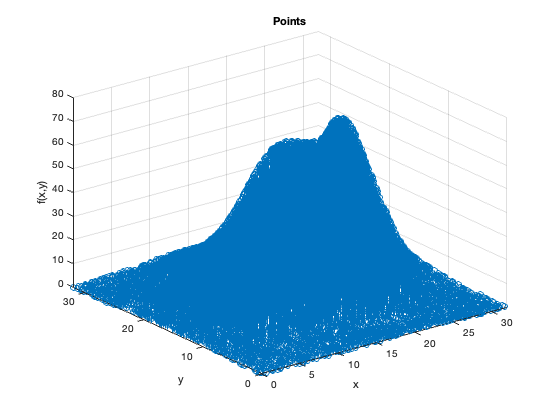
\includegraphics[width=\linewidth]{figures/ex1_stem3.png}
        \caption{Data plot}
        \label{fig:figures/ex1_stem3.png}
    \end{minipage}%
    \begin{minipage}{.5\textwidth}
        \centering
        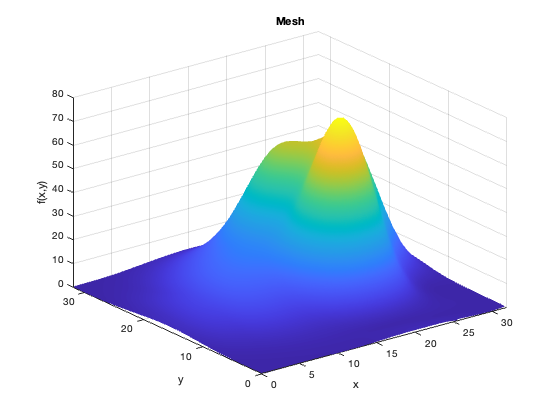
\includegraphics[width=\linewidth]{figures/ex1_mesh.png}
        \caption{Mesh plot}
        \label{fig:figures/ex1_mesh.png}
    \end{minipage}
\end{figure}

\begin{figure}[h!]
    \centering
    \begin{minipage}{.5\textwidth}
        \centering
        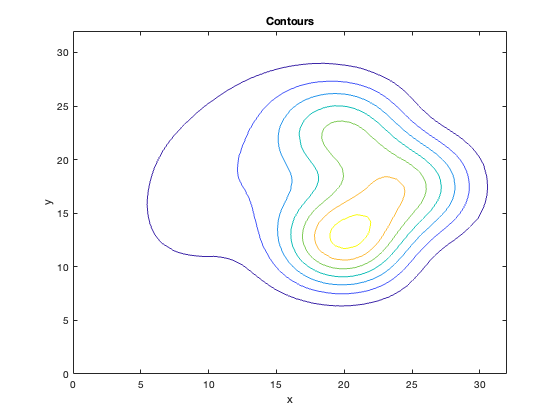
\includegraphics[width=\linewidth]{figures/ex1_contours.png}
        \caption{Contours}
        \label{fig:figures/ex1_contours.png}
    \end{minipage}%
    \begin{minipage}{.5\textwidth}
        \centering
        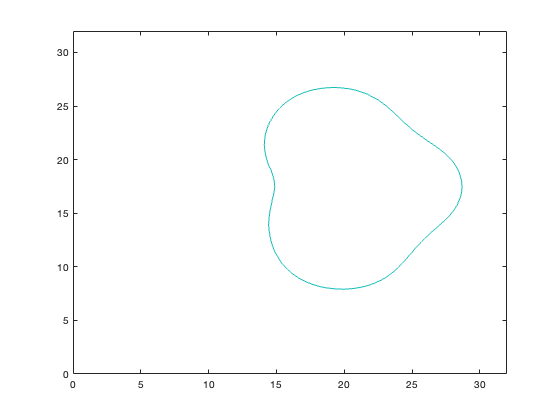
\includegraphics[width=\linewidth]{figures/ex1_alpha_contour.png}
        \caption{$ \alpha = 25 $ contour}
        \label{fig:figures/ex1_alpha_contour.png}
    \end{minipage}
\end{figure}

\begin{verbatim}
area1 =
      201.2490

area2 =
      198.8608

area3 =
      200.6016

area4 =
      201.3788

area5 =
      200.0850
\end{verbatim}

\paragraph{Comments:}
I did several experiments and assuming the real value with $ \alpha =
25 $ is 201, it seems like method 1 provided the most accurate
calculation in most cases. It also seemed like the Monte-Carlo
methods frequently performed the worst.

\bigskip
\hrule

\exercise{Trilateration}

\paragraph{Explanation:}
First I do some basic input validation.
Then, I started by creating an anonymous function to draw circles.
Followed by a loop to allow me to draw an arbitrary amount of circles.
Finally, using the \mttext{fsolve} function I find the intersection
of the first 3 circles.
Using \mttext{axis equal} was important when plotting to get the
correct axis ratio.

\paragraph{MATLAB Code:}

\begin{tiny}
    \verbatiminput{code/trilateration.m}
\end{tiny}

\paragraph{Results:}

\begin{figure}[h!]
    \centering
    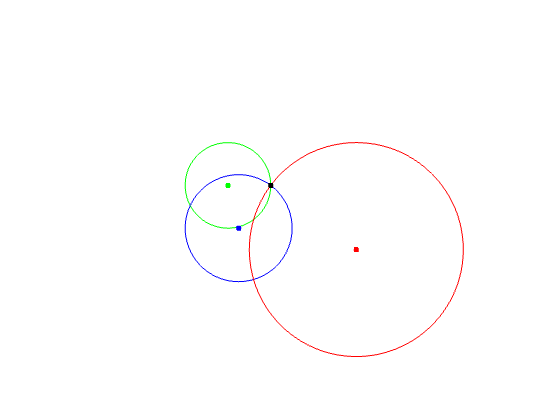
\includegraphics[width=8cm]{figures/ex2.png}
    \caption{Intersection of the 3 circles}
    \label{fig:figures/ex2.png}
\end{figure}

\begin{verbatim}
Intersection:
    x =
            2.1000

    y =
            3.0000
\end{verbatim}

\paragraph{Comments:}
In order to iteratively construct the system of equations, I had to
use a cell array as I could not save anonymous functions in an array.
Additionally, using the \mttext{fsolve} function was non trivial when
using this cell array, requiring me to also use \mttext{cellfun}, as
I needed the same input for each.

\bigskip
\hrule

\exercise{Morse Decoder}

\paragraph{Explanation:}
Again, I start by doing a short input validation.
I continue to doing the sections indicated in the statement.
A brief comment on section 2 is that when plotting the actual first
4000 points, nothing much interesting is seen, however when plotting
4000 equally distances points we already observe the morse pattern as
can be seen in the results section.
I also included a plot of the PSD in decibel scale where we can
immediately see that the tone frequency is approximately $ 750Hz $.
After that, I followed the instructions as they are until I reached
section 6 and had to do the actual decoding.

I started from the approximate derivative calculated in section 5 and
started by smoothing out this signal.
I used \mttext{smoothdata} initially and followed by zeroing out
values that are lower than $ 0.9 * max\_values $.
The goal was to keep one value per maximum as these would indicate a change.
I then keep those indices different than 0 and compute the dots
until this difference first by dividing by the sampling frequency and
then by the dot duration.
I round these numbers and then eliminate those equal to 0.
With this, we have an array of $ \{1, 3, 7\} $.
I then noticed that the odd indices in this array represented 1s and
the even 0s.
So I simply replaced the values by the adequate morse symbol code (.,-, ).

\begin{verbatim}
-- .- .   ..- -. .. - ...--   ..-. .- .-.. .-.. ..--- ....-
\end{verbatim}

Finally, I used the \mttext{morse.mat} given in the previous problem
set to get the letters and find the final translation.

{\bf MAE UNIT3 FALL24}

\paragraph{MATLAB Code:}

\begin{tiny}
    \verbatiminput{code/morse_decoder.m}
\end{tiny}

\paragraph{Results:}

\begin{figure}[H]
    \centering
    \begin{minipage}{.5\textwidth}
        \centering
        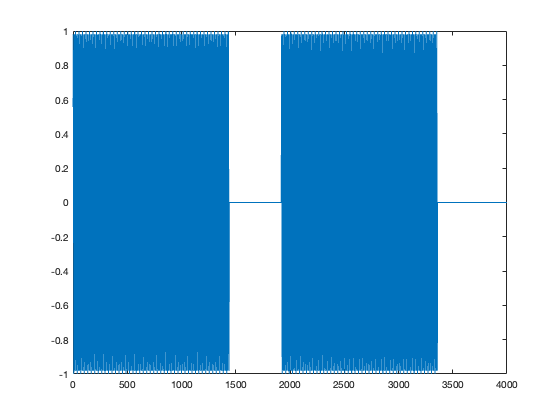
\includegraphics[width=\linewidth]{figures/ex3_firstN.png}
        \caption{Plotting first 4000 points}
        \label{fig:figures/ex3_firstN.png}
    \end{minipage}%
    \begin{minipage}{.5\textwidth}
        \centering
        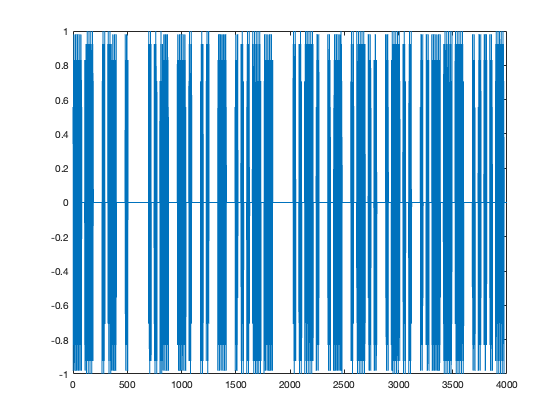
\includegraphics[width=\linewidth]{figures/ex3_N.png}
        \caption{Plotting interpolated 4000 points}
        \label{fig:figures/ex3_N.png}
    \end{minipage}
\end{figure}

\begin{figure}[H]
    \centering
    \begin{minipage}{.5\textwidth}
        \centering
        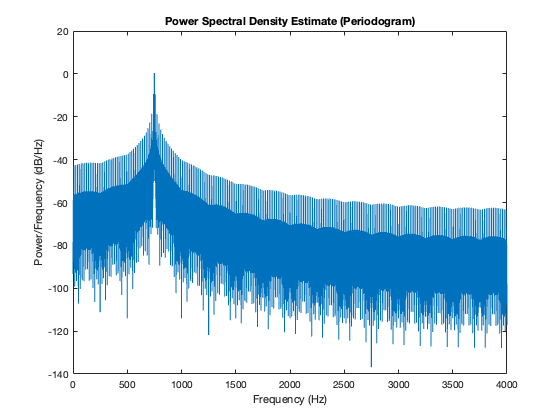
\includegraphics[width=\linewidth]{figures/ex3_psd.png}
        \caption{PSD}
        \label{fig:figures/ex3_psd.png}
    \end{minipage}%
    \begin{minipage}{.5\textwidth}
        \centering
        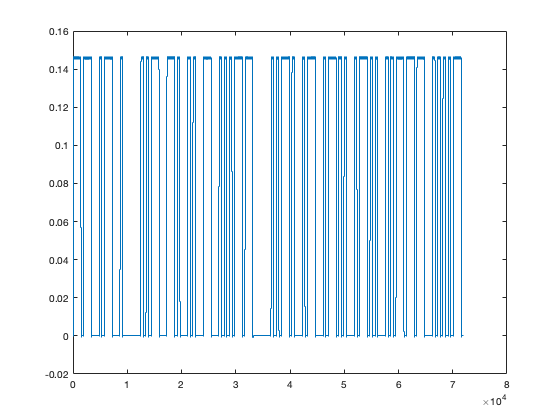
\includegraphics[width=\linewidth]{figures/ex3_bbs.png}
        \caption{Base Band Signal}
        \label{fig:figures/ex3_bbs.png}
    \end{minipage}
\end{figure}

\begin{figure}[H]
    \centering
    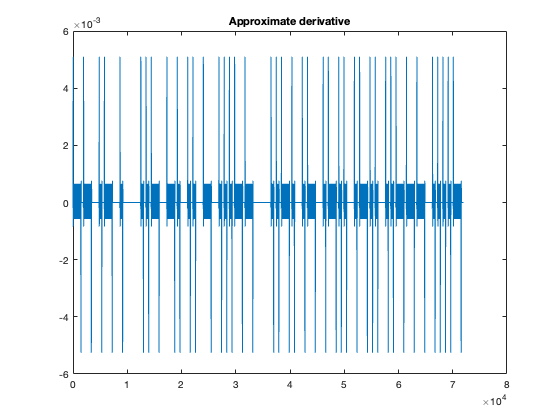
\includegraphics[width=8cm]{figures/ex3_diff.png}
    \caption{Approximating the derivative}
    \label{fig:figures/ex3_diff.png}
\end{figure}

\begin{verbatim}
DECODED SOUND:
    MAE UNIT3 FALL24
\end{verbatim}

\paragraph{Comments:}
I was expecting to find the final decoding harder, but (in my
opinion) thanks to a couple lucky attempts I managed to do it with
the method I mentioned above.
My main stroke of luck was getting the array of $\{1,3,7\}$ with odd
indices representing 1s and evens 0s.

\bigskip
\hrule

